%%%%%%%%%%%%%%%%%%%%%%%%%%%%%%%%%%%%%%%%%
% University/School Laboratory Report
% LaTeX Template
% Version 3.0 (4/2/13)
%
% This template has been downloaded from:
% http://www.LaTeXTemplates.com
%
% Original author:
% Linux and Unix Users Group at Virginia Tech Wiki 
% (https://vtluug.org/wiki/Example_LaTeX_chem_lab_report)
%
% License:
% CC BY-NC-SA 3.0 (http://creativecommons.org/licenses/by-nc-sa/3.0/)
%
%%%%%%%%%%%%%%%%%%%%%%%%%%%%%%%%%%%%%%%%%

%----------------------------------------------------------------------------------------
%	PACKAGES AND DOCUMENT CONFIGURATIONS
%----------------------------------------------------------------------------------------

\documentclass{article}
\usepackage{geometry}
 \geometry{
 a4paper,
 total={210mm,297mm},
 left=20mm,
 right=20mm,
 top=20mm,
 bottom=20mm,
 }

\usepackage{siunitx} % Provides the \SI{}{} command for typesetting SI units
\usepackage{listings}
\usepackage{graphicx} % Required for the inclusion of images
\usepackage{enumerate}
\usepackage{float}
\usepackage{color}
\usepackage{booktabs}

\definecolor{mygreen}{RGB}{28,172,0} % color values Red, Green, Blue
\definecolor{mylilas}{RGB}{170,55,241}

\setlength\parindent{0pt} % Removes all indentation from paragraphs

%\usepackage{times} % Uncomment to use the Times New Roman font

%----------------------------------------------------------------------------------------
%	DOCUMENT INFORMATION
%----------------------------------------------------------------------------------------

\title{Network Security \\ 389.159 - SS 2016} % Title

\author{TEAM 16: Stefan \textsc{Heigl}, Florian \textsc{Wörister}} % Author name

\date{\today} % Date for the report
\begin{document}

\lstset{language=Matlab,
    breaklines=true,
    morekeywords={matlab2tikz},
    keywordstyle=\color{blue},
    morekeywords=[2]{1}, keywordstyle=[2]{\color{black}},
    identifierstyle=\color{black},
    stringstyle=\color{mylilas},
    commentstyle=\color{mygreen},
    showstringspaces=false,
    numbers=left,
    numberstyle={\tiny \color{black}},
    numbersep=9pt,
    emph=[1]{for,end,break},emphstyle=[1]\color{red},
}

\maketitle % Insert the title, author and date

\section*{rep-10}
The code in figure \ref{fig:rep10} generates the plot for the first subtask of this exercise. It generates a plot, showing the \textit{\#pkts/hour}. The only difference to the other subtasks is in line 6 of this code snippet. Here the parameter 3 describes the column index of the data we want to plot. The indices for subtask 2-4 can be seen in table \ref{tab:indices}.
\begin{table}[H]
\center
\begin{tabular}{lr}
\toprule
index & feature name \\
\midrule
2 & \#bytes / hour (daily avg.) \\
4 & \#uIPs / hour (daily avg.) \\
5 & \#uIPd / hour (daily avg.) \\
\bottomrule
\end{tabular}
\caption{Indices for the several dataset features}
\label{tab:indices}
\end{table}
\begin{figure}[H]
\lstinputlisting{./chapters/matlab/team16_ex3_rep10_1.m}
\caption{Matlab code for first subtask of rep-10}
\label{fig:rep10}
\end{figure}

In addition a function was implemented, for plotting a graph, which also deals with the epoch to datenum format conversion. The exact implementation of this function is listed in figure \ref{fig:plotDarkNetData}.

\begin{figure}[H]
\lstinputlisting{./chapters/matlab/plotDarknetData.m}
\caption{Matlab code for the 'plotDarknetData' function}
\label{fig:plotDarkNetData}
\end{figure}

For the normalization we simply loaded every feature set in a separate feature vector and devided it by the vectors max value. In figure \ref{fig:normalization} the normalization is demonstrated on the first feature \(\#pkts/hour\). The smoothing, as described in the exercise description, was implemented in the matlab function 'smoothLine'.

\begin{figure}[H]
\lstinputlisting{./chapters/matlab/team16_ex3_rep10_5_normalization.m}
\caption{Matlab code for the normalization}
\label{fig:normalization}
\end{figure}


\subsection*{Results}
\begin{figure}[H]
\center
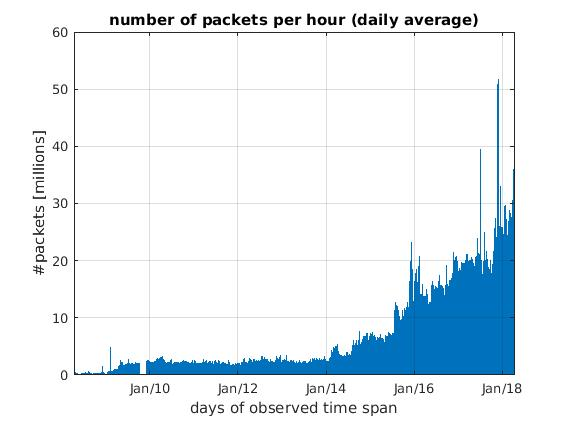
\includegraphics[width=.7\textwidth]{./chapters/plots/rep10_1.jpg}\\
\caption{Results of rep10-1}
\end{figure}
\begin{figure}[H]
\center
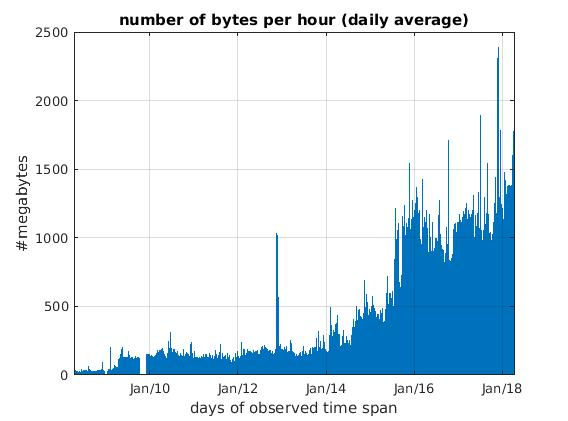
\includegraphics[width=.7\textwidth]{./chapters/plots/rep10_2.jpg}\\
\caption{Results of rep10-2}
\end{figure}
\begin{figure}[H]
\center
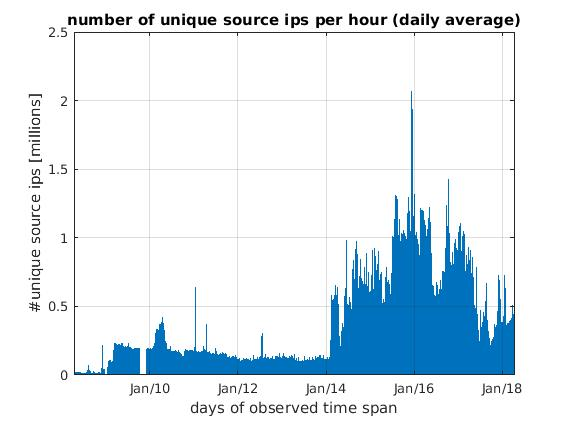
\includegraphics[width=.7\textwidth]{./chapters/plots/rep10_3.jpg}\\
\caption{Results of rep10-3}
\end{figure}
\begin{figure}[H]
\center
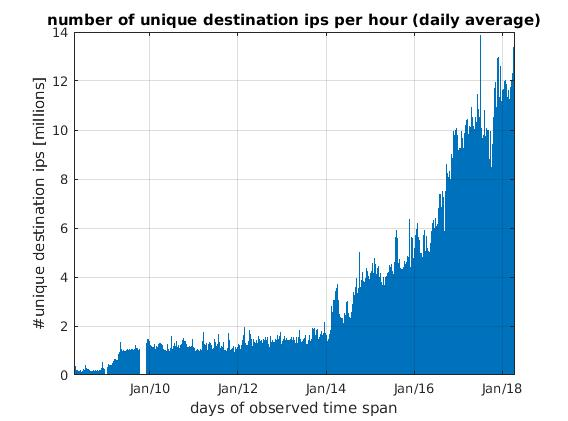
\includegraphics[width=.7\textwidth]{./chapters/plots/rep10_4.jpg}\\
\caption{Results of rep10-4}
\end{figure}

\section*{rep-11}
For this task, the correlation matrix was calculated by executing the matlab code of figure \ref{fig:correlation}
\begin{figure}[H]
\lstinputlisting{./chapters/matlab/team16_ex3_rep11.m}
\caption{Matlab code for the normalization}
\label{fig:correlation}
\end{figure}
The resulting correlation matrix (figure \ref{matrix:correlation}) shows us, that the \text{\#unique source IP addresses per hour} show the lowest correlation values, especially with the \text{\#unique destination IP addresses per hour}


\section*{rep-12}

\section*{rep-13}

\section*{rep-14}

\section*{rep-15}

\section*{rep-16}

\section*{rep-17}

\section*{rep-18}

\section*{rep-19}

\section*{rep-20}

\section*{rep-21}

\section*{rep-22}

\section*{rep-23}


\section*{Exercise 4}
\subsection*{rep-24}
The full command we used for retrieving the \textit{csv} file is listed in figure \ref{fig:bash-flowrec}.
\begin{figure}[H]
\begin{lstlisting}[language=bash]
rwcut --num-recs=200000 --delimited=',' --fields=sIP,dIP,sPort,dPort,protocol,flags,ttl,bytes team16.flowrecord.rw > team16_flowrecord.csv
\end{lstlisting}
\caption{Bash command for retrieving the flow record csv file.}
\label{fig:bash-flowrec}
\end{figure}
\subsection*{rep-25}

\subsection*{rep-26}

\subsection*{rep-27}

\subsection*{rep-28}

\subsection*{rep-29}

\subsection*{rep-30}


\end{document}

